\documentclass{article}
\usepackage{tikz}
\usepackage{pgfplots}
\usepackage{amsmath}

\pgfplotsset{compat=1.18}

\begin{document}

\begin{figure}[htbp]
    \centering
    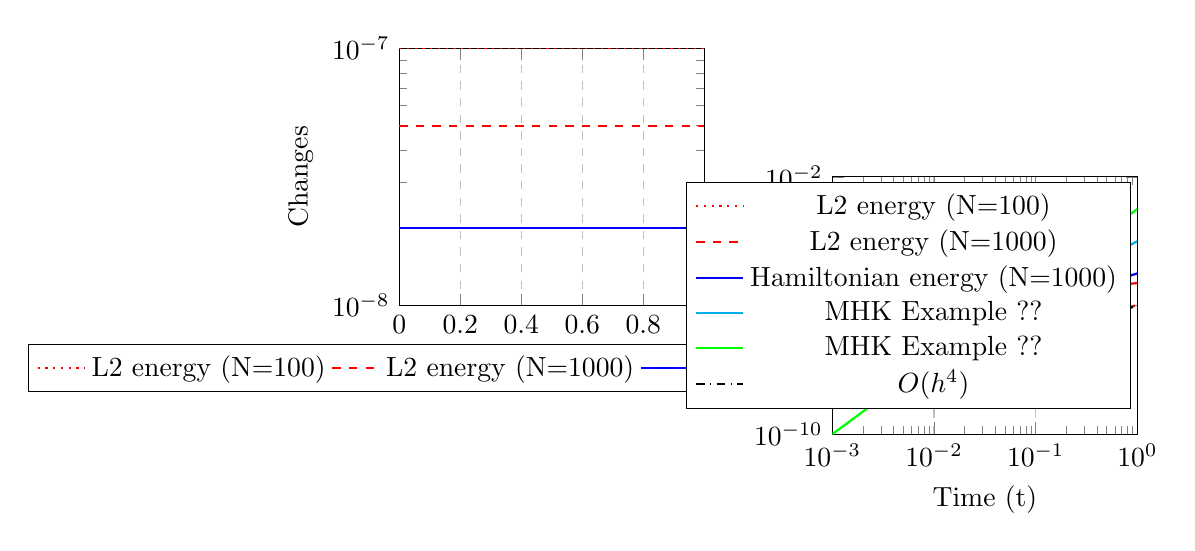
\begin{tikzpicture}
        \begin{axis}[
            width=0.45\textwidth,
            height=0.4\textwidth,
            xlabel={Time (t)},
            ylabel={Changes},
            xmajorgrids,
            ymajorgrids,
            grid style={dashed},
            ymin=1e-8, ymax=1e-7,
            xmin=0, xmax=1,
            ymode=log,
            legend style={at={(0.5,-0.15)}, anchor=north, legend columns=3},
            legend cell align={left}
        ]
            \addplot[red, dotted, thick] coordinates {(0, 1e-7) (1, 1e-7)};
            \addlegendentry{L2 energy (N=100)}
            
            \addplot[red, dashed, thick] coordinates {(0, 5e-8) (1, 5e-8)};
            \addlegendentry{L2 energy (N=1000)}
            
            \addplot[blue, solid, thick] coordinates {(0, 2e-8) (1, 2e-8)};
            \addlegendentry{Hamiltonian energy (N=1000)}
        \end{axis}
        
        \begin{axis}[
            at={(5.5cm,0)},
            anchor=west,
            width=0.45\textwidth,
            height=0.4\textwidth,
            xlabel={Time (t)},
            ylabel={$l_2$ error},
            xmajorgrids,
            ymajorgrids,
            grid style={dashed},
            ymode=log,
            xmode=log,
            ymin=1e-10, ymax=1e-2,
            xmin=1e-3, xmax=1,
        ]
            \addplot[red, dotted, thick] coordinates {(1e-3, 1e-7) (1, 1e-6)};
            \addlegendentry{L2 energy (N=100)}
            
            \addplot[red, dashed, thick] coordinates {(1e-3, 5e-7) (1, 5e-6)};
            \addlegendentry{L2 energy (N=1000)}
            
            \addplot[blue, solid, thick] coordinates {(1e-3, 1e-8) (1, 1e-5)};
            \addlegendentry{Hamiltonian energy (N=1000)}
            
            \addplot[cyan, thick] coordinates {(1e-3, 1e-9) (1, 1e-4)};
            \addlegendentry{MHK Example ??}
            
            \addplot[green, thick] coordinates {(1e-3, 1e-10) (1, 1e-3)};
            \addlegendentry{MHK Example ??}
            
            \addplot[black, dash dot, thick] coordinates {(1e-3, 1e-9) (1, 1e-6)};
            \addlegendentry{$O(h^4)$}
        \end{axis}
    \end{tikzpicture}
\end{figure}

\end{document}